
\begin{knitrout}
\definecolor{shadecolor}{rgb}{0.969, 0.969, 0.969}\color{fgcolor}\begin{kframe}
\begin{alltt}
\hlstd{cpu} \hlkwb{<-} \hlkwd{scan}\hlstd{(}\hlkwc{file}\hlstd{=}\hlstr{"cputime.txt"}\hlstd{)}

\hlcom{# Define the function to compute the natural logarithm of the polulation mean.}
\hlstd{logmean} \hlkwb{<-} \hlkwa{function}\hlstd{(}\hlkwc{data}\hlstd{) \{}
  \hlkwd{return}\hlstd{(}\hlkwd{log}\hlstd{(}\hlkwd{mean}\hlstd{(data)))}
\hlstd{\}}

\hlcom{# Define the resample function.}
\hlstd{resample} \hlkwb{<-} \hlkwa{function}\hlstd{(}\hlkwc{x}\hlstd{) \{}
  \hlkwd{sample}\hlstd{(x,} \hlkwc{size} \hlstd{=} \hlkwd{length}\hlstd{(x),} \hlkwc{replace} \hlstd{=} \hlnum{TRUE}\hlstd{)}
\hlstd{\}}

\hlcom{# Define the bootstrap function.}
\hlstd{rboot} \hlkwb{<-} \hlkwa{function}\hlstd{(}\hlkwc{B}\hlstd{,} \hlkwc{statistic}\hlstd{,} \hlkwc{simulator}\hlstd{,} \hlkwc{data}\hlstd{) \{}
  \hlstd{tboots} \hlkwb{<-} \hlkwd{replicate}\hlstd{(B,} \hlkwd{statistic}\hlstd{(}\hlkwd{simulator}\hlstd{(data)))}
  \hlkwd{return}\hlstd{(tboots)}
\hlstd{\}}

\hlcom{# Define the bootstrap function that directly compute specific statistic.}
\hlstd{bootstrap.se} \hlkwb{<-} \hlkwa{function}\hlstd{(}\hlkwc{B}\hlstd{,} \hlkwc{statistic}\hlstd{,} \hlkwc{simulator}\hlstd{,} \hlkwc{data}\hlstd{) \{}
  \hlstd{tboots} \hlkwb{<-} \hlkwd{rboot}\hlstd{(B, statistic, simulator, data)}
  \hlstd{se} \hlkwb{<-} \hlkwd{sd}\hlstd{(tboots)}
  \hlkwd{return}\hlstd{(se)}
\hlstd{\}}

\hlcom{# Define the bootstrap function that directly compute the bias of specific statistic.}
\hlstd{bootstrap.bias} \hlkwb{<-} \hlkwa{function}\hlstd{(}\hlkwc{B}\hlstd{,} \hlkwc{statistic}\hlstd{,} \hlkwc{simulator}\hlstd{,} \hlkwc{t.hat}\hlstd{,} \hlkwc{data}\hlstd{) \{}
  \hlstd{tboots} \hlkwb{<-} \hlkwd{rboot}\hlstd{(B, statistic, simulator, data)}
  \hlstd{bias} \hlkwb{<-} \hlkwd{mean}\hlstd{(tboots)} \hlopt{-} \hlstd{t.hat}
  \hlkwd{return}\hlstd{(bias)}
\hlstd{\}}

\hlcom{# Define the bootstrap function that directly compute the quantile}
\hlcom{# of specific statistic.}
\hlstd{bootstrap.alphaquantile} \hlkwb{<-} \hlkwa{function}\hlstd{(}\hlkwc{B}\hlstd{,} \hlkwc{statistic}\hlstd{,} \hlkwc{simulator}\hlstd{,} \hlkwc{data}\hlstd{,} \hlkwc{alpha}\hlstd{) \{}
  \hlstd{tboots} \hlkwb{<-} \hlkwd{rboot}\hlstd{(B, statistic, simulator, data)}
  \hlstd{alphaquantile} \hlkwb{<-} \hlkwd{quantile}\hlstd{(tboots, alpha)}
  \hlkwd{return}\hlstd{(alphaquantile)}
\hlstd{\}}

\hlcom{# Define the bootstrap function that directly compute the quantile}
\hlcom{# of the bias of specific statistic.}
\hlstd{bootstrap.alphaquantile.hat} \hlkwb{<-} \hlkwa{function}\hlstd{(}\hlkwc{B}\hlstd{,} \hlkwc{statistic}\hlstd{,} \hlkwc{simulator}\hlstd{,} \hlkwc{t.hat}\hlstd{,} \hlkwc{data}\hlstd{,} \hlkwc{alpha}\hlstd{) \{}
  \hlstd{alphaquantile} \hlkwb{<-} \hlkwd{bootstrap.alphaquantile}\hlstd{(B, statistic, simulator, data, alpha)}
  \hlstd{alphaquantile.hat} \hlkwb{<-} \hlstd{alphaquantile} \hlopt{-} \hlstd{t.hat}
  \hlkwd{return}\hlstd{(alphaquantile.hat)}
\hlstd{\}}

\hlcom{# Define function to compute the CI with normal approximation.}
\hlstd{NormalCI} \hlkwb{<-} \hlkwa{function}\hlstd{(}\hlkwc{B}\hlstd{,} \hlkwc{statistic}\hlstd{,} \hlkwc{simulator}\hlstd{,} \hlkwc{t.hat}\hlstd{,} \hlkwc{data}\hlstd{,} \hlkwc{alpha}\hlstd{) \{}
  \hlstd{tboots} \hlkwb{<-} \hlkwd{rboot}\hlstd{(B, statistic, simulator, data)}
  \hlstd{se} \hlkwb{<-} \hlkwd{sd}\hlstd{(tboots)}
  \hlstd{bias} \hlkwb{<-} \hlkwd{mean}\hlstd{(tboots)} \hlopt{-} \hlstd{t.hat}
  \hlstd{ci.lower} \hlkwb{<-} \hlstd{t.hat} \hlopt{-} \hlstd{bias} \hlopt{-} \hlkwd{qnorm}\hlstd{(}\hlnum{1} \hlopt{-} \hlstd{alpha}\hlopt{/}\hlnum{2}\hlstd{)} \hlopt{*} \hlstd{se}
  \hlstd{ci.upper} \hlkwb{<-} \hlstd{t.hat} \hlopt{-} \hlstd{bias} \hlopt{-} \hlkwd{qnorm}\hlstd{(alpha}\hlopt{/}\hlnum{2}\hlstd{)} \hlopt{*} \hlstd{se}
  \hlkwd{return}\hlstd{(}\hlkwd{list}\hlstd{(}\hlkwc{ci.lower}\hlstd{=ci.lower,}\hlkwc{ci.upper}\hlstd{=ci.upper))}
\hlstd{\}}

\hlcom{# Define function to compute the CI with basic bootstrap.}
\hlstd{BasicBootstrapCI} \hlkwb{<-} \hlkwa{function}\hlstd{(}\hlkwc{B}\hlstd{,} \hlkwc{statistic}\hlstd{,} \hlkwc{simulator}\hlstd{,} \hlkwc{t.hat}\hlstd{,} \hlkwc{data}\hlstd{,} \hlkwc{alpha}\hlstd{) \{}
  \hlstd{tboots} \hlkwb{<-} \hlkwd{rboot}\hlstd{(B, statistic, simulator, data)}
  \hlstd{ci.lower} \hlkwb{<-} \hlnum{2} \hlopt{*} \hlstd{t.hat} \hlopt{-} \hlkwd{quantile}\hlstd{(tboots,} \hlnum{1} \hlopt{-} \hlstd{alpha}\hlopt{/}\hlnum{2}\hlstd{)}
  \hlstd{ci.upper} \hlkwb{<-} \hlnum{2} \hlopt{*} \hlstd{t.hat} \hlopt{-} \hlkwd{quantile}\hlstd{(tboots, alpha}\hlopt{/}\hlnum{2}\hlstd{)}
  \hlkwd{return}\hlstd{(}\hlkwd{list}\hlstd{(}\hlkwc{ci.lower}\hlstd{=ci.lower,}\hlkwc{ci.upper}\hlstd{=ci.upper))}
\hlstd{\}}

\hlcom{# Define function to compute the CI with percentile bootstrap.}
\hlstd{PercentileBootstrapCI} \hlkwb{<-} \hlkwa{function}\hlstd{(}\hlkwc{B}\hlstd{,} \hlkwc{statistic}\hlstd{,} \hlkwc{simulator}\hlstd{,} \hlkwc{data}\hlstd{,} \hlkwc{alpha}\hlstd{) \{}
  \hlstd{tboots} \hlkwb{<-} \hlkwd{rboot}\hlstd{(B, statistic, simulator, data)}
  \hlstd{ci.lower} \hlkwb{<-} \hlkwd{quantile}\hlstd{(tboots, alpha}\hlopt{/}\hlnum{2}\hlstd{)}
  \hlstd{ci.upper} \hlkwb{<-} \hlkwd{quantile}\hlstd{(tboots,} \hlnum{1} \hlopt{-} \hlstd{alpha}\hlopt{/}\hlnum{2}\hlstd{)}
  \hlkwd{return}\hlstd{(}\hlkwd{list}\hlstd{(}\hlkwc{ci.lower}\hlstd{=ci.lower,}\hlkwc{ci.upper}\hlstd{=ci.upper))}
\hlstd{\}}

\hlcom{# Compute t.hat}
\hlstd{t.hat} \hlkwb{<-} \hlkwd{logmean}\hlstd{(cpu)}

\hlcom{# Compute bootstrap distribution.}
\hlstd{cpu.boot} \hlkwb{<-} \hlkwd{rboot}\hlstd{(}\hlnum{1000}\hlstd{, logmean, resample, cpu)}

\hlcom{# Compute standard error of theta hat.}
\hlstd{t.hat.se} \hlkwb{<-} \hlkwd{bootstrap.se}\hlstd{(}\hlnum{1000}\hlstd{, logmean, resample, cpu)}

\hlcom{# Compute bias of theta hat.}
\hlstd{t.hat.bias} \hlkwb{<-} \hlkwd{bootstrap.bias}\hlstd{(}\hlnum{1000}\hlstd{, logmean, resample,} \hlkwd{logmean}\hlstd{(cpu), cpu)}

\hlcom{# Compute 2.5th and 97.5th percentiles of the theta hat.}
\hlkwd{bootstrap.alphaquantile}\hlstd{(}\hlnum{1000}\hlstd{, logmean, resample, cpu,} \hlnum{0.025}\hlstd{)}
\end{alltt}
\begin{verbatim}
##     2.5%
## 3.692207
\end{verbatim}
\begin{alltt}
\hlkwd{bootstrap.alphaquantile}\hlstd{(}\hlnum{1000}\hlstd{, logmean, resample, cpu,} \hlnum{0.975}\hlstd{)}
\end{alltt}
\begin{verbatim}
##    97.5%
## 4.050683
\end{verbatim}
\begin{alltt}
\hlcom{# Compute 2.5th and 97.5th percentiles of the bias of theta hat.}
\hlkwd{bootstrap.alphaquantile.hat}\hlstd{(}\hlnum{1000}\hlstd{, logmean, resample,} \hlkwd{logmean}\hlstd{(cpu), cpu,} \hlnum{0.025}\hlstd{)}
\end{alltt}
\begin{verbatim}
##       2.5%
## -0.1946992
\end{verbatim}
\begin{alltt}
\hlkwd{bootstrap.alphaquantile.hat}\hlstd{(}\hlnum{1000}\hlstd{, logmean, resample,} \hlkwd{logmean}\hlstd{(cpu), cpu,} \hlnum{0.975}\hlstd{)}
\end{alltt}
\begin{verbatim}
##     97.5%
## 0.1838178
\end{verbatim}
\begin{alltt}
\hlcom{# Compute normal approximation of CI.}
\hlkwd{NormalCI}\hlstd{(}\hlnum{1000}\hlstd{, logmean, resample,} \hlkwd{logmean}\hlstd{(cpu), cpu,} \hlnum{0.05}\hlstd{)}
\end{alltt}
\begin{verbatim}
## $ci.lower
## [1] 3.692305
##
## $ci.upper
## [1] 4.06934
\end{verbatim}
\begin{alltt}
\hlcom{# Compute basic bootstrap CI.}
\hlkwd{BasicBootstrapCI}\hlstd{(}\hlnum{1000}\hlstd{, logmean, resample,} \hlkwd{logmean}\hlstd{(cpu), cpu,} \hlnum{0.05}\hlstd{)}
\end{alltt}
\begin{verbatim}
## $ci.lower
##    97.5%
## 3.689361
##
## $ci.upper
##     2.5%
## 4.067459
\end{verbatim}
\begin{alltt}
\hlcom{# Compute normal approximation of CI.}
\hlkwd{PercentileBootstrapCI}\hlstd{(}\hlnum{1000}\hlstd{, logmean, resample, cpu,} \hlnum{0.05}\hlstd{)}
\end{alltt}
\begin{verbatim}
## $ci.lower
##     2.5%
## 3.668655
##
## $ci.upper
##    97.5%
## 4.044892
\end{verbatim}
\begin{alltt}
\hlcom{# Draw histogram and qqplot for bootstrap distribution}
\hlcom{# Create fig folder to store plot.}
\hlkwa{if}\hlstd{(}\hlopt{!}\hlkwd{dir.exists}\hlstd{(}\hlstr{"fig"}\hlstd{))} \hlkwd{dir.create}\hlstd{(}\hlstr{"fig"}\hlstd{)}
\hlkwd{pdf}\hlstd{(}\hlstr{"fig/hist.pdf"}\hlstd{,} \hlkwc{width}\hlstd{=}\hlnum{5}\hlstd{,} \hlkwc{height}\hlstd{=}\hlnum{7}\hlstd{)}
\hlkwd{hist}\hlstd{(cpu.boot)}
\hlkwd{dev.off}\hlstd{()}
\end{alltt}
\begin{verbatim}
## pdf
##   2
\end{verbatim}
\begin{alltt}
\hlkwd{pdf}\hlstd{(}\hlstr{"fig/qqplot.pdf"}\hlstd{,} \hlkwc{width}\hlstd{=}\hlnum{5}\hlstd{,} \hlkwc{height}\hlstd{=}\hlnum{7}\hlstd{)}
\hlkwd{qqnorm}\hlstd{(cpu.boot)}
\hlkwd{qqline}\hlstd{(cpu.boot)}
\hlkwd{dev.off}\hlstd{()}
\end{alltt}
\begin{verbatim}
## pdf
##   2
\end{verbatim}
\begin{alltt}
\hlcom{# Verification}
\hlkwd{library}\hlstd{(boot)}
\hlstd{nlm.hat} \hlkwb{<-} \hlkwa{function}\hlstd{(}\hlkwc{x}\hlstd{,} \hlkwc{indices}\hlstd{)\{}
  \hlstd{result} \hlkwb{<-} \hlkwd{log}\hlstd{(}\hlkwd{mean}\hlstd{(x[indices]))}
  \hlkwd{return}\hlstd{(result)}
\hlstd{\}}
\hlstd{nlm.hat.boot} \hlkwb{<-} \hlkwd{boot}\hlstd{(cpu, nlm.hat,} \hlkwc{R} \hlstd{=} \hlnum{1000}\hlstd{,} \hlkwc{sim} \hlstd{=} \hlstr{"ordinary"}\hlstd{,} \hlkwc{stype} \hlstd{=} \hlstr{"i"}\hlstd{)}
\hlkwd{names}\hlstd{(nlm.hat.boot)}
\end{alltt}
\begin{verbatim}
##  [1] "t0"        "t"         "R"         "data"      "seed"
##  [6] "statistic" "sim"       "call"      "stype"     "strata"
## [11] "weights"
\end{verbatim}
\begin{alltt}
\hlkwd{log}\hlstd{(}\hlkwd{mean}\hlstd{(cpu))}
\end{alltt}
\begin{verbatim}
## [1] 3.87605
\end{verbatim}
\begin{alltt}
\hlstd{nlm.hat.boot}\hlopt{$}\hlstd{t0}
\end{alltt}
\begin{verbatim}
## [1] 3.87605
\end{verbatim}
\begin{alltt}
\hlkwd{mean}\hlstd{(nlm.hat.boot}\hlopt{$}\hlstd{t)} \hlopt{-} \hlstd{nlm.hat.boot}\hlopt{$}\hlstd{t0}
\end{alltt}
\begin{verbatim}
## [1] -0.007910493
\end{verbatim}
\begin{alltt}
\hlkwd{quantile}\hlstd{(}\hlkwd{mean}\hlstd{(nlm.hat.boot}\hlopt{$}\hlstd{t)} \hlopt{-} \hlstd{nlm.hat.boot}\hlopt{$}\hlstd{t0,}\hlnum{0.975}\hlstd{)}
\end{alltt}
\begin{verbatim}
##        97.5%
## -0.007910493
\end{verbatim}
\begin{alltt}
\hlkwd{sd}\hlstd{(nlm.hat.boot}\hlopt{$}\hlstd{t)}
\end{alltt}
\begin{verbatim}
## [1] 0.1015838
\end{verbatim}
\begin{alltt}
\hlkwd{plot}\hlstd{(nlm.hat.boot)}
\end{alltt}
\end{kframe}
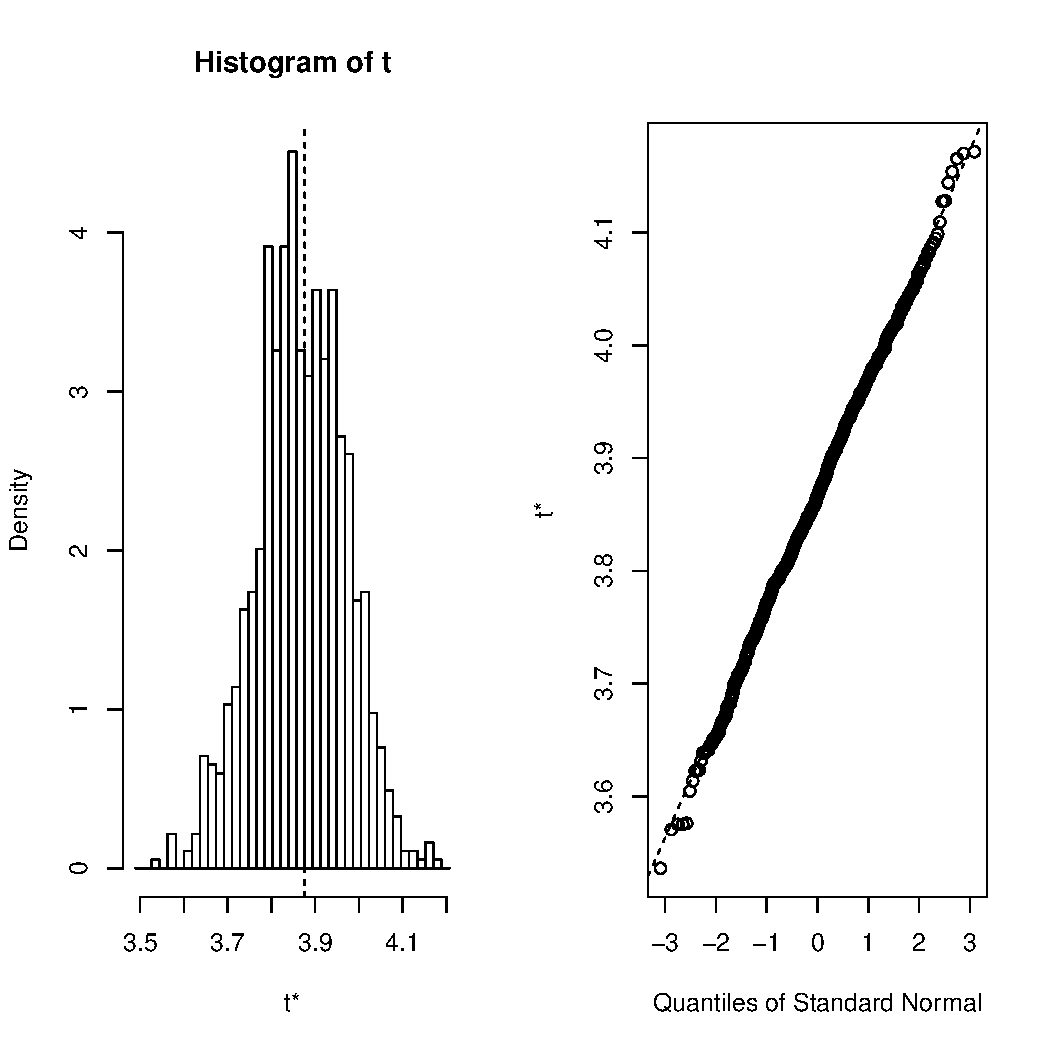
\includegraphics[width=\maxwidth]{figure/Test-1}
\begin{kframe}\begin{alltt}
\hlkwd{boot.ci}\hlstd{(nlm.hat.boot)}
\end{alltt}


{\ttfamily\noindent\color{warningcolor}{\#\# Warning in boot.ci(nlm.hat.boot): bootstrap variances needed for studentized intervals}}\begin{verbatim}
## BOOTSTRAP CONFIDENCE INTERVAL CALCULATIONS
## Based on 1000 bootstrap replicates
##
## CALL :
## boot.ci(boot.out = nlm.hat.boot)
##
## Intervals :
## Level      Normal              Basic
## 95%   ( 3.685,  4.083 )   ( 3.695,  4.095 )
##
## Level     Percentile            BCa
## 95%   ( 3.657,  4.057 )   ( 3.690,  4.091 )
## Calculations and Intervals on Original Scale
\end{verbatim}
\end{kframe}
\end{knitrout}

